\chapter{Describing Distributions with Numbers}

\section{Outlier}
One term that is important for discussions in this chapter is \textbf{outlier}. An \textbf{outlier} is a data point that differs significantly from other observations in a dataset. It can be unusually large or small compared to the rest of the data.

Outliers are \textbf{relative} because what qualifies as an outlier in one dataset may not be an outlier in another. For example, consider the ages of five students in a high school: 15, 16, 14, 16, and 24. Here, the age 24 is much larger than the rest of the data, making it an \textbf{outlier}. In another context, such as a dataset of graduate students’ ages, 24 might be typical and not considered an outlier.

\section{Resistant}
A numerical summary of observations is called \textbf{resistant} if \textbf{outliers} (extreme observations) have little, if any, influence on its value.

\section{Measures of Center}
\textbf{Measures of center} tell us where the center or the middle of the data set is. We are interested in the \textbf{mean}, \textbf{median} and \textbf{mode}.

\subsection{Mean}
The \textbf{mean} is the sum of the observations divided by the number of observations. It is interpreted as the balance point of the distribution. The \textbf{mean} is denoted as $\bar{x}$ and is affected by the presence of \textbf{outliers}. Therefore, the \textbf{mean} is not a \textbf{resistant measure}. The formula for the \textbf{mean} is

\[
\text{Mean} = \bar{x} = \frac{\sum_{i=1}^n x_i}{n}
\]

where
\begin{itemize}
    \item \( x_i \) represents each individual value in the dataset
    \item \( n \) is the total number of values in the dataset
    \item \( \sum \) denotes the summation symbol, meaning you add up all the \( x_i \) values
\end{itemize}

\subsubsection*{How to Calculate the Mean}
\begin{enumerate}
    \item Add all the values in the dataset together.
    \item Divide the total by the number of values in the dataset.
\end{enumerate}

\subsubsection*{Example on How to Calculate the Mean}
Suppose you have the dataset: \( 3, 7, 8, 10, 12 \).

\[
\bar{x} = \frac{\sum_{i=1}^n x_i}{n} = \frac{3 + 7 + 8 + 10 + 12}{5} = \frac{40}{5} = 8
\]

So, the mean is \( 8 \).

\subsection{Median}
The \textbf{median} is the middle value of the observations when the observations are ordered from the smallest to the largest (or from the largest to the smallest). The \textbf{median} is not affected by the presence of \textbf{outliers}. Therefore, the median is a \textbf{resistant measure}.

\subsubsection*{How to Find the Median}
\begin{enumerate}
    \item Arrange all observations in ascending or descending order.
    \item Determine the number of observations, \(n\).
    \item Locate the position of the median:
    \begin{itemize}
        \item If \(n\) is odd, the median is the observation at position \((n+1)/2\).
        \item If \(n\) is even, the median is the average of the two middle observations at positions \(n/2\) and \((n/2) + 1\).
    \end{itemize}
\end{enumerate}

\subsubsection*{Example 1 on How to Calculate the Median}
Suppose you have the dataset: \( 10, 25, 15, 20, 30 \).
\begin{enumerate}
    \item Arrange: \(10, 15, 20, 25, 30\).
    \item \(n = 5\) (odd), so the median is at position \((5+1)/2 = 3\).
\end{enumerate}

Therefore, the median is \( 20 \).

\subsubsection*{Example 2 on How to Calculate the Median}
Suppose you have the dataset: \( 10, 15, 30, 20, 25, 35 \).
\begin{enumerate}
    \item Arrange: \(10, 15, 20, 25, 30, 35\).
    \item \(n = 6\) (even), so the median is the average of the two middle values at positions \(6/2 = 3\) and \((6/2) + 1 = 4\).
\end{enumerate}

Therefore, the median is \( = (20 + 25)/2 = 22.5 \).

\subsection{Mode}
The \textbf{mode} is the value or values that appear most frequently in a dataset. The \textbf{mode} is not affected by the presence of \textbf{outliers}. Therefore, the median is a \textbf{resistant measure}.

\subsubsection*{How to Find the Mode}
\begin{enumerate}
    \item List all the values in the dataset.
    \item Count how many times each value appears.
    \item Identify the value(s) with the highest frequency.
\end{enumerate}

\subsubsection*{Example 1 on How to Calculate the Mode}
Suppose you have the dataset: \(1, 2, 2, 3, 4, 4, 4, 5\). A count of each value gives us this: 
\[
\begin{array}{c|l}
\textbf{Value} & \textbf{Frequency} \\
\hline
1 & 1 \\
2 & 2 \\
3 & 1 \\
4 & 3 \\
5 & 1 \\
\end{array}
\]

Therefore, the mode is \( 4 \) (appears most frequenctly). 

\subsubsection*{Example 2 on How to Calculate the Mode}
Suppose you have the dataset: \( \text{“red," “blue," “red," “green," “red," “blue"} \). A count of each value gives us this: 
\[
\begin{array}{c|l}
\textbf{Value} & \textbf{Frequency} \\
\hline
\text{red} & 3 \\
\text{blue} & 2 \\
\text{green} & 1 \\
\end{array}
\]

Therefore, the mode is “red" (appears most frequenctly). 

\section{Mean, Median, and Skewness}
The shape of a distribution influences whether the mean is larger or smaller than the median. For instance, an extremely large value out in the right-hand tail pulls the mean to the right. The mean then usually falls above the median.

When a distribution is close to symmetric, the tails will be of similar length, and therefore the median and mean are similar. For skewed distributions, the mean lies toward the direction of skew (the longer tail) relative to the median, as Figure \ref{fig:skewness.jpg} shows. This is because extreme observations in a tail affect the balance point for the distribution, which is the mean. The more highly skewed the distribution, the more the mean and median tend to differ.

\begin{figure}[h!]
\centering
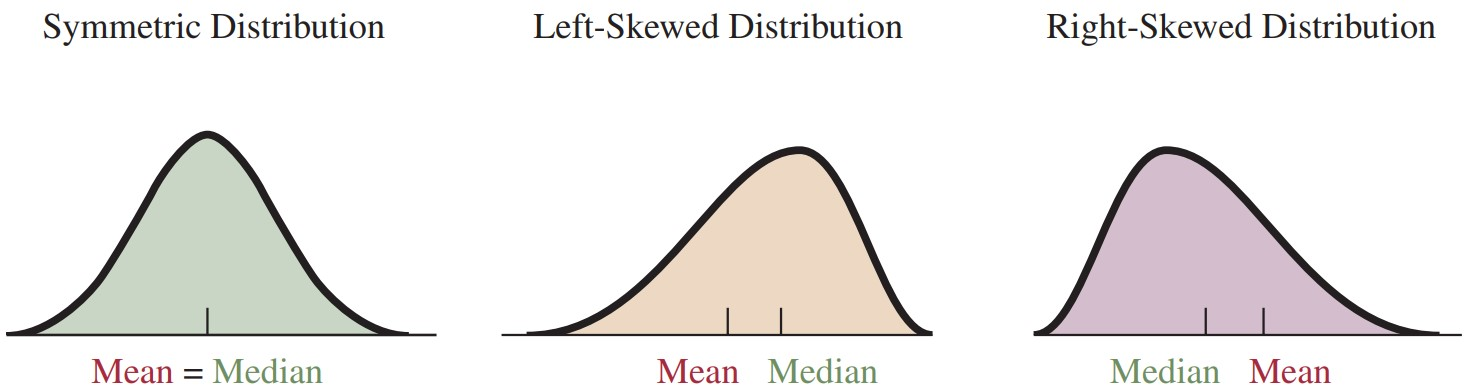
\includegraphics[width=1\textwidth]{figures/skewness.jpg}
\caption{Relationship Between the Mean and Median}
\label{fig:skewness.jpg}
\end{figure}

Generally, if the shape is
\begin{itemize}
    \item perfectly symmetric, the mean equals the median.
    \item skewed to the left, the mean is smaller than the median.
    \item skewed to the right, the mean is larger than the median.
\end{itemize}

\section{Measures of Variability}
\textbf{Measures of variability} tell us the degree of variation among the values in the given data. We are interested in the \textbf{range}, \textbf{quartiles}, \textbf{interquartile range}, \textbf{variance}, and \textbf{standard deviation}.

\subsection{Range}
The \textbf{range} is the difference between the largest (maximum) and smallest (minimum) observations. \textbf{Range} is affected by the presence of outliers. Therefore, range is \textbf{not} a resistant measure.

\subsubsection*{Example 1 on How to Calculate the Range}
Suppose you have the dataset: \( 9, 13, 7, 11, 21, 10, 23, 19, 35 \).
The minimum observation is 7, and the maximum observation is 35. Therefore, the range is \( = 35 - 7 = 28 \).

\subsection{Quartiles}
The quartiles split the distribution into four parts, each containing one quarter (25\%) of the observations. See Figure \ref{fig:quartiles.jpg}.

\begin{itemize}
    \item First quartile (Q1): It separates the lowest 25\% from the upper 75\%. Q1 is the median of the lower half of the data.
    \item Second quartile (Q2, Median): It separates the lower 50\% from the upper 50\%. Q2 is the median of the entire data.
    \item Third quartile (Q3): It separates the lower 75\% from the upper 25\%. Q3 is the median of the upper half of the data.
\end{itemize}


\begin{figure}[h!]
\centering
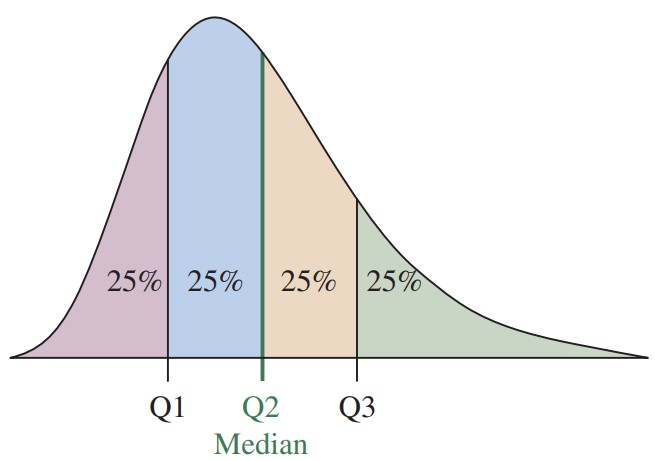
\includegraphics[width=0.5\textwidth]{figures/quartiles.jpg}
\caption{The Quartiles Split the Distribution Into Four Parts. Twenty-five percent is below the first quartile (Q1), 25\% is between the first quartile and the second quartile (Q2, the median), 25\% is between the second quartile and the third quartile (Q3), and 25\% is above the third quartile.}
\label{fig:quartiles.jpg}
\end{figure}

\subsection{Interquartile Range (IQR)}
It is the distance between the first and third quartiles: \(IQR = Q3 - Q1\).

\subsection{The \(\bm{1.5 \times IQR}\) Rule for Identifying Outliers}
The IQR can be used to identify outliers. An observation is a suspected outlier if it falls more than \((1.5 \times IQR)\) above \(Q3\) or below \(Q1\). That is 
\begin{enumerate}
    \item observations less than \(Q1-(1.5 \times IQR)\) are suspected outliers
    \item observations greater than \(Q3+(1.5 \times IQR)\) are suspected outliers
\end{enumerate}

\subsubsection*{Example 1 on Quartiles, Interquartile Range, and Outlier Detection}
Consider the data set: 16, 35, 31, 22, 28, 25, 26, 22, 30, 23, 31. Are there any outliers?

\begin{enumerate}
    \item Arrange the data set in order; from the lowest to the highest:
\[
16, \ 22, \ 22, \ 23, \ 25, \ 26, \ 28, \ 30, \ 31, \ 31, \ 35
\]
    \item Find the main Median (Q2). There are 11 (odd) observations, so there’s only one middle number. The middle number is the 6\textsuperscript{th} observation. That is \(26\). Therefore, the main \textbf{median} \( (Q2) = 26 \).
    
    \item Find Q1: \( Q1 \) is the median of the observations that are below the main median (\( Q2 \)). The observations are: \( 16, \ 22, \ 22, \ 23, \ 25 \). We have 5 observations (odd), so there’s only one middle number. The middle number is \( 22 \).
Therefore, the first quartile \( Q1 = 22 \).

    \item Find the third quartile (Q3): \( Q3 \) is the median of the observations that are above the main median (\( Q2 \)). The observations are: \( 28, \ 30, \ 31, \ 31, \ 35 \). We have 5 observations (odd), so there’s only one middle number. The middle number is \(31\). Therefore, the third quartile \( Q3 = 31 \).

    \item Calculate the IQR: \(IQR = Q3 - Q1 = 31 - 22 = 9\).
    \item Lower Boundary for Outliers: \(Q1 - (1.5 \times IQR) = 22 - (1.5 \times 9) = 22 - 13.5 = 8.5\). Observations less than 8.5 are suspected outliers. We note that none of the observations is less than 8.5.

    \item Upper Boundary for Outliers: \( Q3 + (1.5 \times IQR) = 31 + (1.5 \times 9) = 31 + 13.5 = 44.5 \). Observations greater than or above 44.5 are suspected outliers. We note that none of the observations is greater than 44.5.
\end{enumerate}

Therefore, there are no suspected outliers.

\subsection{Variance and Standard Deviation}
Although it is good practice to mention the smallest and largest value when describing the distribution of a variable, we usually don’t use the range to measure variability. A much better numerical summary of variability uses all the data, and it describes a typical distance of how far the data falls from the mean. It does this by summarizing \textbf{deviations} from the mean.

The \textbf{deviation} of an observation \(x\) from the mean \(\bar{x}\) is \( (x - \bar{x}) \), the difference between the observation and the sample mean.

The sum (and therefore the mean) of the deviations always equals zero, regardless of the actual data values. Hence, summary measures of variability from the mean use either the \textbf{squared deviations} or their absolute values.

The average of the squared deviations is called the \textbf{variance}. Because the variance uses the square of the units of measurement for the original data, its square root is easier to interpret. This is called the \textbf{standard deviation}. In summary, the \textbf{standard deviation} is the square root of the \textbf{variance}; and they both measure the average distance the observations are from the mean.

The \textbf{Variance} is denoted as \( s^2 \) while the \textbf{Standard Deviation} is denoted as \( s \).

\[
\text{Variance} = s^2 = \frac{1}{n-1} \sum (x_i - \bar{x})^2 = \frac{(x_1-\bar{x})^2 + (x_2-\bar{x})^2 + \cdots + (x_n-\bar{x})^2}{n-1} 
\]

\[
\text{Standard Deviation} = s = \sqrt{s^2} = \sqrt{\frac{1}{n-1} \sum (x_i - \bar{x})^2}
\]

\subsection*{Note:}
\begin{enumerate}
    \item Both the variance and standard deviation are \textbf{nonnegative}. That is \( s^2 \geq 0 \) and \( s \geq 0 \).
    \item Since we use the mean (\( \bar{x} \)) to compute the variance and standard deviation, they are affected by the presence of outliers. That is, the \textbf{variance} and \textbf{standard deviation} are not \textbf{resistant} to outliers.
\end{enumerate}

\subsubsection*{Example 1 on Variance and Standard Deviation Calculation}

Given the ages (in years) of 5 students below, find the variance and standard deviation of their ages: \(18, \ 17, \ 21, \ 17, \ 22\).

\[
\bar{x} = \frac{1}{n} \sum_{i=1}^{n} x_i = \frac{1}{5} (18 + 17 + 21 + 17 + 22) = \frac{1}{5} (95) = 19
\]

\textbf{Mean} = 19 years

\vspace{0.2cm}

\textbf{Table of Deviations and Squared Deviations}

\[
\begin{array}{|c|c|c|}
\hline
x_i & x_i - \bar{x} & (x_i - \bar{x})^2 \\ \hline
18 & -1 & 1 \\ \hline
17 & -2 & 4 \\ \hline
21 & 2 & 4 \\ \hline
17 & -2 & 4 \\ \hline
22 & 3 & 9 \\ \hline
\end{array}
\]

\[
\sum_{i=1}^{5} (x_i - \bar{x})^2 = 22
\]

\vspace{0.2cm}

\textbf{Variance Calculation}

\[
s^2 = \frac{1}{n-1} \sum_{i=1}^{n} (x_i - \bar{x})^2
\]

\[
s^2 = \frac{1}{5-1} (22) = \frac{22}{4} = 5.5
\]

\textbf{Variance} = \( 5.5 \, \text{years}^2 \)

\vspace{0.2cm}

\textbf{Standard Deviation Calculation}
\[
s = \sqrt{s^2} = \sqrt{5.5} \approx 2.345
\]

\textbf{Standard Deviation} = \( 2.345 \, \text{years} \)

\section{The Five-Number Summary}
The \textbf{five-number summary} of a data set consists of the minimum value, first quartile Q1, 
median, third quartile Q3, and the maximum value.

The \textbf{five-number summary} is the basis of a graphical display called the \textbf{box 
plot}. The box of a box plot contains the central 50\% of the distribution, from the 
first quartile to the third quartile (see the figure below). 

A line inside the box marks the \textbf{median}. A line goes from the lower end of the box to the smallest observation that is not a potential outlier. A separate line goes from the upper end of the box to the largest observation that is not a potential outlier. These lines are called \textbf{whiskers}. The potential outliers (more than 1.5 IQR below the first quartile or above the third quartile) are shown separately with special symbols (such as a dot or a star).

\begin{figure}[h!]
\centering
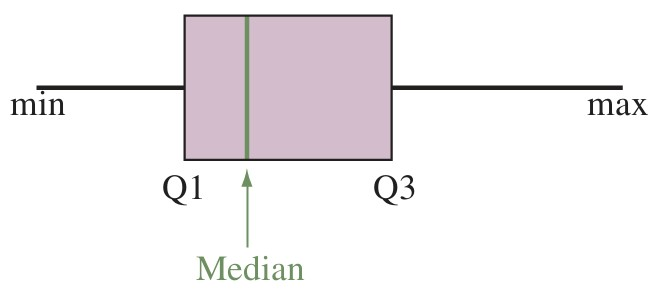
\includegraphics[width=0.5\textwidth]{figures/box_plot.jpg}
\caption{Example of a Box Plot}
\label{fig:box_plot.jpg}
\end{figure}

\subsection{Skewness in a Box Plot}
\begin{itemize}
    \item When Q2 is closer to Q1, we have a right-skewed box plot.
    \item When Q2 is closer to Q3, we have a left-skewed box plot.
\end{itemize}

\subsection{The Box Plot Compared with the Histogram}

\textbf{A box plot does not portray certain features of a distribution, such as distinct mounds and possible gaps, as clearly as a histogram}. For example, the histogram and box plot (Figure \ref{fig:histogram_box_plot.jpg}) refer to the same data, the waiting time between eruptions of the Old Faithful geyser in Yellowstone National Park. The histogram suggests that the distribution is bimodal (two distinct mounds), but we could not learn this from the box plot. This comparison shows that more than one type of graph may be needed to summarize a data set well.

A box plot does indicate skew from the relative lengths of the whiskers and the two parts of the box. The side with the larger part of the box and the longer whisker usually has skew in that direction. However, the box plot will not show us whether there is a large gap in the distribution contributing to the skew. But, as we’ve seen, \textbf{box plots are useful for identifying potential outliers}. 

\begin{figure}[h!]
\centering
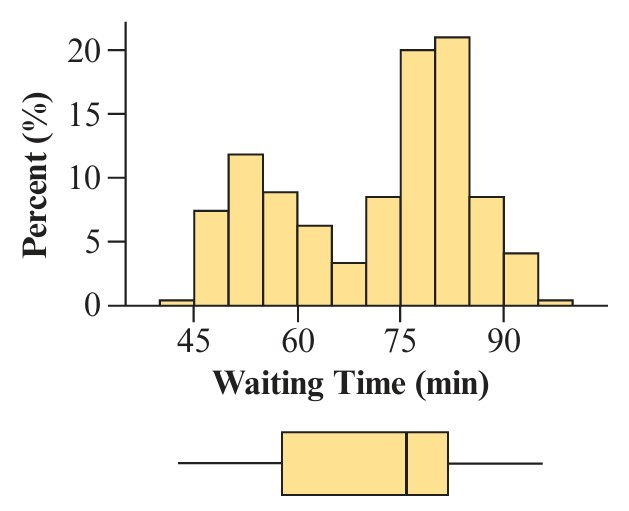
\includegraphics[width=0.5\textwidth]{figures/histogram_box_plot.jpg}
\caption{Histogram compared to Box Plot}
\label{fig:histogram_box_plot.jpg}
\end{figure}




 

 